

\lecture{Hypothesis Testing With Two Dependent Samples}{hypothesis-testing-two-dep}
\section{Hypothesis Testing With Two Dependent Samples}

\title{Hypothesis Testing With Two Dependent Samples}
\subtitle{Is there a difference?}

%\author{Kelly Black}
%\institute{Clarkson University}
\date{7 November 2014}

\begin{frame}
  \titlepage
\end{frame}

\begin{frame}
  \frametitle{Outline}
  \tableofcontents[hideothersubsections,sectionstyle=show/hide]
\end{frame}



\subsection{Clicker Quiz}


\begin{frame}
  \frametitle{Clicker Quiz}

  % \begin{clickerQuiz}

  \iftoggle{clicker}{%

    A group of twenty people from St. Lawrence County, NY have their
    blood stream cholesterol levels tested. The borderline high level
    is 200 mg/dL. The sample mean of the group is 205 mg/dL with a
    sample standard deviation of 15 mg/dL. Is the mean cholesterol
    level for the county above the borderline high level?

    What hypothesis test would you form to test this? \\
    ~ \\
    \begin{tabular}{ll@{\hspace{3em}}l}
      A & $H_0$: The mean is 200 mg/dL  \\
        & $H_a$: The mean is above 200 mg/dL  \\
      ~ \\
      B & $H_0$: The mean is 200 mg/dL \\ 
        & $H_a$: The mean is less than 200 mg/dL \\
      ~ \\
      C & $H_0$: The mean is 200 mg/dL \\ 
        & $H_a$: The mean is not 200 mg/dL 
    \end{tabular}

  }

  %\end{clickerQuiz}
  

\end{frame}

\subsection{Differences Between Groups}

\begin{frame}{Comparing Two Groups}

  We have two populations and take some samples: \\
  \begin{columns}[T]
    \column{.3\textwidth}
      \begin{tabular}{ll}
        Group 1 \\ \hline
        $x_1$  \\
        $x_2$  \\
        $x_3$  \\
        $\vdots$ \\
        $x_{\redText{N}}$  \\
      \end{tabular}

    \uncover<2>{%
      \vfill

      \blueText{This is the $X$ variable.}
    }

    \vfill
    \column{.3\textwidth}
    \begin{tabular}{ll}
      Group 2 \\ \hline
      $y_1$ \\
      $y_2$ \\
      $y_3$ \\
      \\
      $\vdots$ \\
      $\vdots$ \\
      \\
      $y_{\redText{M}}$ \\
    \end{tabular}

    \uncover<2>{%
      \vfill

      \blueText{This is the $Y$ variable.}
    }

    \column[t]{.4\textwidth}

    \vfill

    Are they different? 

    \vfill

    What does that question even mean? 

    \vfill

    What is different?

    \vfill

  \end{columns}


\end{frame}

\begin{frame}{Example I}

  Group one takes a medication that we think might reduce blood stream
  cholesterol levels. Group two takes a medication that we think will
  not do anything.

  \vfill

  Does the first medication make a difference?

  \vfill

  \only<2->{\redText{These are independent samples.}}
  
\end{frame}

\begin{frame}{Example II}

  A group of people will have their blood stream cholesterol levels
  tested. They will then be given a drug that we think will reduce
  their cholesterol levels. We test their blood levels at a later
  time.

  \vfill

  Did the medication make a difference?

  \vfill

  \only<2->{\redText{These are dependent samples.}}
  
\end{frame}

\begin{frame}{Independent vs. Independent Samples}

  \begin{columns}[T]
    \column{.5\textwidth}
    Independent Samples

    \includegraphics[width=5cm]{img/independentSamples}

    \vfill
    \column{.5\textwidth}

    Dependent Samples

    \begin{tabular}{l@{$\Rightarrow$}r}
      ``Before'' & ``After'' \\ \hline
      $\textrm{before}_1$  & $\textrm{after}_1$ \\
      $\textrm{before}_2$  & $\textrm{after}_2$ \\
      $\textrm{before}_3$  & $\textrm{after}_3$ \\
      $\vdots$ & $\vdots$ \\
      $\textrm{before}_{\redText{N}}$ & $\textrm{after}_{\redText{N}}$  \\
    \end{tabular}


    \vfill

  \end{columns}

  
\end{frame}

\subsection{Differences Between Dependent Samples}


\begin{frame}{Dependent Samples}

  We have one populations and take two samples on the same subjects: \\
  \begin{columns}
    \column{.5\textwidth}
    \begin{tabular}{ll}
      ``Before'' & ``After'' \\ \hline
      $x_1$  & $y_1$ \\
      $x_2$  & $y_2$ \\
      $x_3$  & $y_3$ \\
      $\vdots$ & $\vdots$ \\
      $x_{\redText{N}}$ & $y_{\redText{N}}$  \\
    \end{tabular}
    \column{.5\textwidth}
    \only<2->{%
      Define a new random variable, $W=X-Y$: \\
      \begin{tabular}{ll}
        W \\ \hline
        $x_1-y_1$ \\
        $x_2-y_2$ \\
        $x_3-y_3$ \\
        $\vdots$ \\
        $x_{\redText{N}}-y_{\redText{N}}$ \\
      \end{tabular}
    }
  \end{columns}


\end{frame}

\begin{frame}{Dependent Samples}

  \begin{itemize}
  \item We have two random variables, $X$ and $Y$.
  \item There is a direct relationship between them.
  \item We \textbf{CAN} define $W=X-Y$. (i.e. subtraction makes
    sense.)
  \item We define specific samples of $W$:
    \begin{eqnarray*}
      w_i & = & x_i - y_i.
    \end{eqnarray*}
  \item We can now analyze $W$ in the exact same way we did with a
    single variable.
  \end{itemize}
  
\end{frame}

\begin{frame}{Example}

  An additive is developed for hydraulic fluid. Ten samples are taken,
  and the viscosity is measured. The additive is added and the
  viscosity is measured again. Did it make a difference?

  \begin{columns}
    \column{.67\textwidth}

    \begin{tabular}{ll}
      w/o additive (c/P) & w/ additive (c/P)  \\\hline
      4.1 & 4.1 \\
      2.0 & 1.9 \\
      3.9 & 3.8 \\
      6.0 & 5.9 \\
      2.3 & 2.3 \\
      4.1 & 4.0 \\
      7.4 & 7.3 \\
      3.2 & 3.1 \\
      4.3 & 4.2 \\
      3.5 & 3.4
    \end{tabular}

    \column{.33\textwidth}

    \only<2->{%
    \begin{tabular}{l@{=}l}
      X-Y  \\ \hline
      4.1-4.1 & 0.0 \\
      2.0-1.9 & 0.1 \\
      3.9-3.8 & 0.1 \\
      6.0-5.9 & 0.1 \\
      2.3-2.3 & 0.0 \\
      4.1-4.0 & 0.1 \\
      7.4-7.3 & 0.1 \\
      3.2-3.1 & 0.1 \\
      4.3-4.2 & 0.1 \\
      3.5-3.4 & 0.1
    \end{tabular}

    % w <- c(0,.1,.1,.1,0,.1,.1,.1,.1,.1)

    }

  \end{columns}
  
\end{frame}

%%% Local Variables: 
%%% mode: latex
%%% TeX-master: t
%%% End: 
